% Paper text, shared by main.tex (PNAS template, for Overleaf) and preview.tex (plain two-column preview that compiles here).
% DRAFT 26 Nov 2026: BERTopic part only. The tone (emotion) work is being redone and the network analyses are not in this draft yet (marked TODO). Plan and numbers: REPORT_PLAN.md and seedoils/PLAN.md.
% Limit: 6 pages including figures and references. Every number comes from themes_final_summary_v3.csv, prob_outlier_reduction.csv, figures_bertopic.py or a script in seedoils/notebooks.
% Macros used below (\matmethods, \showmatmethods, \dropcap) exist in the PNAS class and are stubbed in preview.tex. Title, abstract, significance statement, author contributions: meta.tex.

\dropcap{I}n 2024 the Reddit community built around the claim that seed oils are toxic grew about threefold, and its conversation turned towards politics. What did that community talk about before and after the surge, and which topics gave way?

\section*{Introduction}
Online health communities are where contested claims about food are argued out, yet we rarely see how the conversation of such a community changes when it suddenly grows. r/StopEatingSeedOils, a subreddit devoted to the claim that seed oils (soybean, canola, sunflower and similar) harm health, is a clean case: posts and comments per year rose from 39{,}454 in 2023 to 118{,}433 in 2024. We ask a descriptive question: what was discussed before and after the surge, which topics grew, which shrank, and when? We do not ask what caused the surge.

We answer it with a topic model of 149{,}815 comments and self-posts, grouped by hand into 14 themes. Topic modelling of text with BERTopic \cite{grootendorst2022bertopic} and LDA \cite{blei2003lda} is standard; the step of turning topics into categories by reading them, and setting cut-offs by reading samples, is adapted from Kardos \cite{kardos2023unsupervised}, and the design of setting online opinion against what is known comes from an analysis of sleep-training claims by The Pudding (TODO: cite). The theme scheme, the outlier rule and the hand checks are ours, and we report them as design choices with checks next to each claim.

In short: politics, vaccines and distrust of industry grew, fatty-acid biochemistry shrank, and the political wave faded within a year.

% \Endparasplit ends the first-page column setting from main.tex: move it to the end of the paragraphs that fill the first page.
\Endparasplit

\section*{Results}
\subsection*{The conversation moved from fatty-acid chemistry towards politics, vaccines and distrust}
Of the 149{,}815 documents, 106{,}715 (71.2\%) sit in a theme under our outlier rule (Methods); the same share is kept before and after 2024. Politics grew from 0.65\% of themed documents before 2024 to 3.21\% from 2024 ($\times$4.9), vaccines and COVID from 0.32\% to 1.14\% ($\times$3.5), distrust of industry, medicine and media from 3.25\% to 5.90\% ($\times$1.8) and ingredient labels from 2.37\% to 3.39\% ($\times$1.4) (Fig.~\ref{fig:themes}B). Fatty-acid biochemistry (omega-6 and PUFA) fell from 19.1\% to 12.8\% ($\times$0.67) and keto, carbs and fasting from 7.9\% to 5.5\% ($\times$0.69). Eight other themes moved by less than 20\%, including shopping ($\times$1.13), specific oils ($\times$1.09) and lifestyle ($\times$1.01).

The timing differs by theme (Fig.~\ref{fig:themes}A). Politics averaged 0.7\% of themed documents in 2023, 7.2\% from August to December 2024 (peak 14.1\% in November 2024), 2.3\% in 2025 and 1.1\% in January to October 2026. Vaccines followed the same shape (0.3\%, 1.8\%, 0.9\%, 0.4\%). Distrust rose and stayed above its starting level (3.5\%, 6.9\%, 5.1\%, 4.9\%). Biochemistry fell to 10.0\% in late 2024 and recovered to 14.4\% in 2026, so the loss is partly temporary.

\begin{figure*}[t]\centering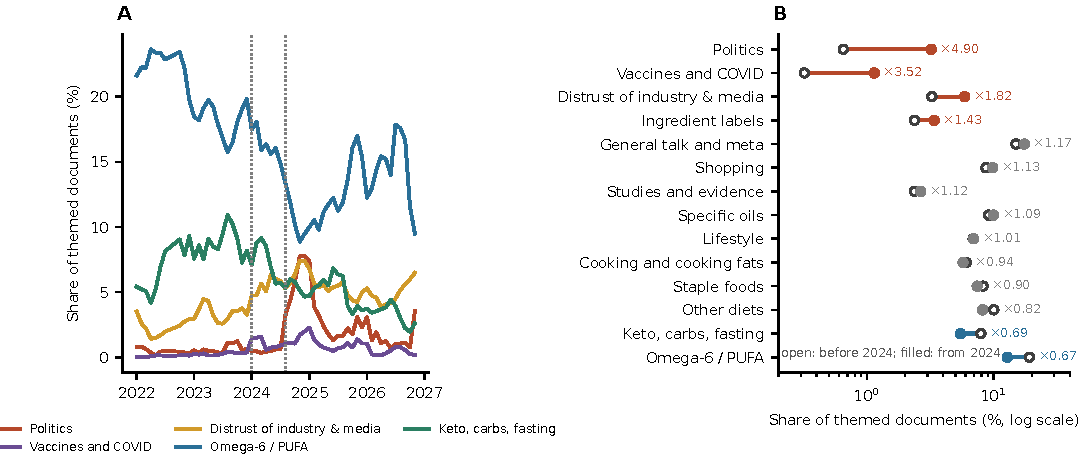
\includegraphics[width=\textwidth]{figures/fig1_themes.pdf}
\caption{\textbf{What the community talked about before and after the 2024 surge.} (A) Monthly share of themed documents in r/StopEatingSeedOils for the five themes that changed most (growth ratio furthest from 1; the other nine are in B), as a 3-month mean; dotted lines mark January and August 2024. (B) Share of themed documents before 2024 (open) and from 2024 (filled) for all 14 themes on a log axis, with the ratio; red marks growth above 1.25 and blue decline below 0.8. Politics and vaccines rise sharply and fade within a year (A), while fatty-acid biochemistry falls and partly recovers. Themes are hand-assigned groups of 123 BERTopic topics; documents without a confident topic (28.8\%) are left out.}\label{fig:themes}\end{figure*}

\subsection*{The pattern holds under other outlier rules; its size, for politics, does not}
BERTopic leaves 38.8\% of documents as outliers. Under four ways of handling them (all moved to the nearest topic, or moved only if their topic probability is at least 0.02, 0.05 or 0.10) the direction of every theme's change is the same, and ratios move by 0.1 or less for all themes except vaccines (3.1 to 3.6) and politics (3.6 to 5.4) (Fig.~\ref{fig:checks}A). A second method, LDA with 123 topics, agrees only in part: its topics are less coherent (NPMI 0.06--0.07 against 0.25) and match BERTopic weakly (AMI 0.22); with its topics mapped to the initial themes it also finds omega-6 falling and distrust rising in most runs, but politics rises much less (about 0.2--0.4\% to 0.3--0.7\% across three seeds), while at 30 topics politics does rise (1.1\% to 2.3\%).

The hand check qualifies the outlier rule. One author judged 90 comments just above and just below the 0.05 threshold (15 per theme and side, three themes, side hidden). Comments moved into a topic fit their theme no better than those left out (62\% against 60\%); only for politics is there a clear gap (100\% against 73\%, difference +27 points, interval +7 to +53) (Fig.~\ref{fig:checks}B). We therefore use the outlier threshold as a sensitivity check and not as a confidence filter.

\begin{figure*}[t]\centering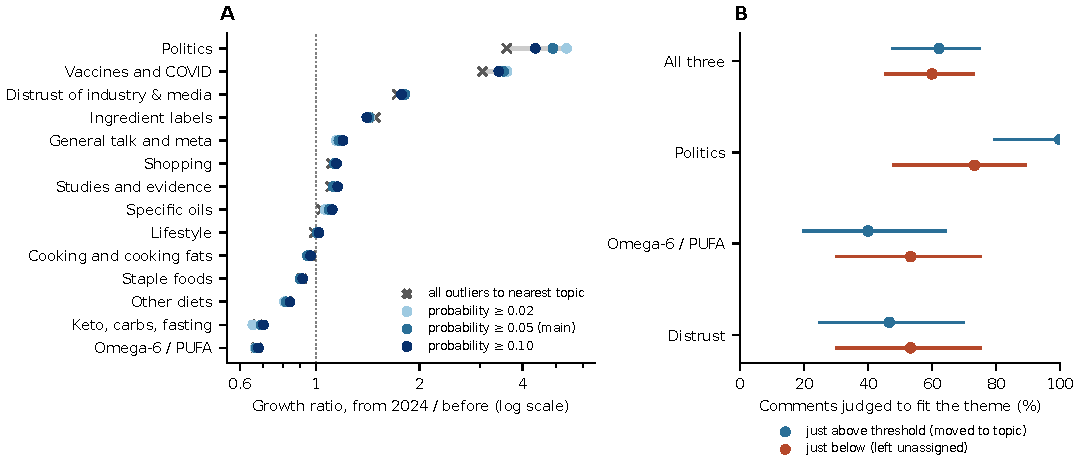
\includegraphics[width=\textwidth]{figures/fig2_checks.pdf}
\caption{\textbf{Checks on the theme result.} (A) Growth ratio (from 2024 divided by before) for each theme under four outlier rules; the grey bar spans the four values. Directions agree everywhere; only politics and vaccines change size. (B) Hand check: share of 15 comments per theme and side judged to fit the theme, just above the 0.05 threshold (moved to a topic) and just below (left unassigned), with 95\% intervals. Above is no better than below except for politics, so the threshold is a sensitivity check. One labeller, preliminary theme scheme.}\label{fig:checks}\end{figure*}

\subsection*{TODO}
TODO: commenter network and community results, and the tone results, are not part of this draft.

\section*{Discussion}
Between 2023 and 2024 the conversation about seed oils in this community shifted from the chemistry of fatty acids towards politics, vaccines and distrust of industry and medicine. Politics and vaccines were a wave that peaked in late 2024 and faded within a year; distrust stayed above its starting level; the biochemistry theme fell and partly recovered. That fits a community whose growth brought in other concerns, and it shows that the change was not a permanent replacement of the original topics.

What the result does not mean: it does not show what caused the surge, because we describe documents, not people or reasons; it does not say that new members, rather than existing ones, wrote the political comments, which needs a separate analysis; and it says nothing about tone or emotion, which we have not analysed here. A topic model measures what a document is about; it misses how it is said, who says it, and documents that mix several subjects (each document gets one topic).

The limitations we found ourselves are three. First, the 14 themes are hand-made. They began as nine themes drafted with an AI assistant and were extended and refined by reading topic words and comments, so the sizes of the changes depend on the scheme: adding or removing one borderline topic moved the politics ratio between 3.6 and 6.1 in earlier versions. We therefore report the direction of each change with confidence and its size as a range. Second, 28.8\% of documents have no confident topic and are left out, and our hand check shows that moving them into topics does not improve fit except for politics. Third, the hand check is small (15 comments per theme and side, one labeller, a preliminary scheme). A convincing next step is a second labeller and a larger sample.

Outliers and small counts matter most for politics and vaccines. About half of the politics documents (52\%) are outliers that our rule moved into a topic, only 160 politics documents (in 81 threads) fall before 2024, and the ratio of $\times$4.9 has a 95\% interval of 3.1 to 7.8 when threads are resampled; for vaccines only 12\% are moved-in outliers but just 79 documents fall before 2024 (interval 2.3 to 6.0). Distrust of industry, medicine and media rests on 795 documents before 2024 and is far more stable ($\times$1.8, interval 1.5 to 2.2). Growth is therefore secure for all three themes (every interval excludes 1), but the size is only well determined for distrust. Wrongly assigned documents would affect the small before-2024 count most; because such documents add to the before-share, they would make the growth ratio too low and not too high. We did not read the politics documents before 2024 to measure how many are misassigned, so we cannot rule it out, and we report the sizes for politics and vaccines as ranges. The intervals cover sampling noise only, not the outlier rule or the theme scheme.

\matmethods{
\textbf{Data.} We collected all posts and comments of r/StopEatingSeedOils (243{,}223 comments, 11{,}648 posts) and r/ScientificNutrition (177{,}989 comments, 14{,}282 posts) from the Arctic Shift archive, a per-subreddit Pushshift-style Reddit archive \cite{baumgartner2020pushshift}, on 22 November 2026 (the last days are incomplete). Accounts named AutoModerator or ending in ``bot'' were removed. The text corpus is every comment and self-post of at least 15 words after removing quoted lines and URLs: 149{,}815 documents for r/StopEatingSeedOils (142{,}894 comments, 6{,}921 self-posts, 19{,}356 authors, median 35 words); this draft analyses r/StopEatingSeedOils only. \\
\textbf{Topic model.} Each document was embedded with all-MiniLM-L6-v2 \cite{reimers2019sbert}, reduced to five dimensions with UMAP (cosine, seed 42) \cite{mcinnes2018umap} and clustered with HDBSCAN (minimum cluster size 150, minimum samples 15) \cite{campello2013hdbscan}, as in BERTopic \cite{grootendorst2022bertopic}. Topics are labelled by their ten highest class-based TF-IDF words after lowercasing, removing stop words, merging hand-checked names and terms, marking ``no''/``without'' plus a noun phrase (e.g.\ no\_preservative) and reducing plural nouns to singular; this cleaning changes labels only, not which documents belong to a topic. The model found 123 topics. HDBSCAN left 38.8\% of documents (58{,}186) without a topic. Following the BERTopic documentation, we moved an outlier to its most probable topic only if that soft-clustering probability was at least 0.05 (15{,}086 documents); the other 43{,}100 (28.8\%) stay unassigned and are left out of the theme results. This leaves 106{,}715 documents (71.2\%) in a theme, and the same share is kept before and after 2024 (70.7\% and 71.4\%). \\
\textbf{Themes.} We turn topics into categories by human reading, an approach we adapt from Kardos \cite{kardos2023unsupervised}: a topic model is fitted without labels, a person reads the topics and decides which ones define a category, and the cut-off for assigning documents is set by reading samples. We assigned all 123 topics to 14 themes by hand. Nine initial themes were drafted with an AI coding assistant (Claude Code) and confirmed by one author; we extended and refined them by reading topic words and comments, so the scheme is a design choice and not a grouping derived from the data. Two checks: 46 of 122 topics are closer to another theme's embedding centroid than to their own (median gap 0.046), and document-level agreement with a hierarchical (Ward) grouping of the topic centroids is AMI 0.65 for 14 groups and 0.70 for 22 groups \cite{vinh2010ami}. Theme shares are shares of themed documents; the growth ratio is the share from 2024 divided by the share before 2024. \\
% Tone scoring (GoEmotions) removed from this draft: the emotion analysis is being redone.
\textbf{Networks.} TODO. \\
\textbf{Thread trees.} TODO (numbers in REPORT\_PLAN.md). Rule to state: a bot or deleted/removed comment is dropped only if nobody replied to it, repeated until none is left; if it has replies it stays as a connector so the thread is not cut in two, but is not counted as an author (Reddit's own display rule). \\
\textbf{Checks.} Topic stability: five UMAP seeds gave AMI 0.81 (0.78--0.85) between topic assignments. A second method, LDA ($K{=}123$, three seeds) \cite{blei2003lda}, had lower coherence (NPMI 0.06--0.07 against 0.25) and agreed only weakly with BERTopic (AMI 0.22). Outlier threshold: results were recomputed at 0.02 and 0.10 and with all outliers moved to the nearest topic. Hand check, following Kardos's practice of reading samples at the cut-off \cite{kardos2023unsupervised}: one author judged 90 comments just above or just below the threshold (15 per theme and side, side hidden, three themes, preliminary theme scheme) as fitting their theme or not; 62\% fit above and 60\% below (politics 100\% against 73\%), so the threshold is a sensitivity check and not a confidence filter. TODO: network checks.
}

\showmatmethods{}


\bibliography{references}
